\documentclass{ctexart}
\usepackage{amsmath}
\usepackage{geometry}
\usepackage{color}
\usepackage{diagbox}
\usepackage{lmodern}
\usepackage{listings}
\usepackage{fontspec}
\usepackage{graphicx}
\usepackage{longtable}
\usepackage[titletoc]{appendix}
\usepackage{lipsum}
\usepackage[colorlinks,linkcolor = black]{hyperref}

\newcommand{\blue}{\textcolor{blue}}
\newcommand{\rotate}{\rotatebox{90}}


\definecolor{mygreen}{rgb}{0,0.6,0}
\definecolor{mygray}{rgb}{0.5,0.5,0.5}
\definecolor{mymauve}{rgb}{0.58,0,0.82}
\lstset{ %
backgroundcolor=\color{white},   % choose the background color
basicstyle=\ttfamily,        % size of fonts used for the code
columns=fullflexible,
breaklines=true,                 % automatic line breaking only at whitespace
captionpos=b,                    % sets the caption-position to bottom
tabsize=4,
commentstyle=\color{mygreen},    % comment style
escapeinside={\%*}{*)},          % if you want to add LaTeX within your code
keywordstyle=\color{blue},       % keyword style
stringstyle=\color{mymauve}\ttfamily,     % string literal style
frame=single,
% rulesepcolor=\color{red!20!green!20!blue!20},
% identifierstyle=\color{red},
% language=c++,
}

\geometry{left = 3cm,right = 3cm,top = 2.5cm, right = 2.5cm}

\begin{document}
	\title{数字逻辑与处理器基础实验 \\ 32位MIPS处理器设计}
	\author{孙伟艺\thanks{无52 2015011010}\\ 白钦博\thanks{无52 2015010996} \\ 王敏虎 \thanks{无52 2015011003}}
	\date{\today}
	\maketitle
	\clearpage

	\section{实验目的}
	\begin{itemize}
		\item 熟悉现代处理器的基本工作原理
		\item 掌握单周期和流水线处理器的设计方法
	\end{itemize}

	\section{设计方案}
		\subsection{ALU}
			(孙伟艺)
		\subsection{单周期数据通路}
			(孙伟艺)
		\subsection{流水线数据通路}
		流水线的数据通路由单周期改进而来,主要的改变是在每个流水级之间增加段间寄存器,另外对于各种冒险加上对应冒险检测电路。如图\ref{pipeline1}。

		\begin{figure}[ht]
		\centering
		\includegraphics[width = \textwidth]{pipeline.png}
		\caption{流水线数据通路}
		\label{pipeline1}
		\end{figure}

		\subsubsection{段间寄存器}

		\begin{enumerate}
			\item \verb"IF_ID"段

			该段用来保存指令的PC值和具体指令,故设置如下三个寄存器

\begin{lstlisting}[language = verilog]
reg [31:0] IF_ID_PC;
reg [31:0] IF_ID_PC4;
reg [31:0] IF_ID_ins;
\end{lstlisting}

			\item \verb"ID_EX"段
			
			该段用来保存此条指令产生的各种控制信号、送入ALU的数据,以及其他部分信号,具体为

\begin{lstlisting}[language = verilog]
reg [31:0] ID_EX_CONBA;
reg [31:0] ID_EX_DATA_1;
reg [31:0] ID_EX_DATA_2;
reg [31:0] ID_EX_PC4;
reg [31:0] ID_EX_IMM;
reg [4:0] ID_EX_Rt;
reg [4:0] ID_EX_shamt;
reg [2:0] ID_EX_PCSrc;
reg [4:0] ID_EX_AddrC;
reg [1:0] ID_EX_MemToReg;
reg [5:0] ID_EX_ALUFun;
reg ID_EX_RegWr,ID_EX_ALUSrc1,ID_EX_ALUsrc2,ID_EX_Sign,ID_EX_MemWr,ID_EX_MemRd;
\end{lstlisting}

			\item \verb"EX_MEM"段

			该段主要保存ALU计算的结果及后续需要的控制信号,具体为			

\begin{lstlisting}[language = verilog]
reg [31:0] EX_MEM_PC4;
reg [31:0] EX_MEM_ALUOUT;
reg [31:0] EX_MEM_DATA2;
reg [4:0] EX_MEM_AddrC;
reg [1:0] EX_MEM_MemToReg;
reg EX_MEM_RegWr,EX_MEM_MemWr,EX_MEM_MemRd;
\end{lstlisting}

			\item \verb"MEM_WB"段

			该段保存最后WB段需要的少数几个信号,具体为

\begin{lstlisting}[language = verilog]
reg [31:0] MEM_WB_DATAOUT;
reg [4:0] MEM_WB_AddrC;
reg MEM_WB_RegWr;
\end{lstlisting}
			
			\end{enumerate}

			\subsubsection{冒险检测电路}

			\begin{enumerate}
\item Forward unit	

我们组采用的转发电路与理论课上讲的略有不同,观察我的数据通路可知,转发单元转发数据输入的两个多路选择器在ID段,而理论课讲的此多路选择器在EX段,这样做的原因是在后面优化主频的时候,发现关键路径在通过ALU,也就是说关键路径在EX段,若能减少EX段的slack则主频必定能得到优化,故将这两个多路复用器移到ID段,另外不将ALUSrc1,ALUSrc2控制的两个多路复用器一起移到ID段的原因是,经过这样的尝试发现主频不升反降,关键路径发生了不可预测的变化,所以未做此改动。

转发的具体电路分为三级转发,因为将转发部分移到了ID段,所有的转发条件用到的段间寄存器比理论课都要向前移一段,具体来说

\begin{enumerate}
\item 第一级转发

转发条件为

\begin{lstlisting}[language = verilog]
(EX_MEM_RegWr&&(EX_MEM_AddrC!=0)&&(EX_MEM_AddrC==Rs)&&(ID_EX_AddrC!=Rs||~ID_EX_RegWr))
\end{lstlisting}

转发数据为DataBusC

\item 第二级转发
\begin{lstlisting}[language = verilog]
(ID_EX_RegWr&&(ID_EX_AddrC!=0)&&(ID_EX_AddrC==Rs))
\end{lstlisting}

转发数据为ALUOut

\item 第三级转发

按照理论课所讲的只存在两级转发,因为在理论课中寄存器是先写后读的,故不存在WB段需要转发的问题,但上网查阅后发现,如果实现的时候真的分别用上升沿和下降沿读写寄存器,会出现不稳定的问题,故采用三级转发

转发条件为:
\begin{lstlisting}[language = verilog]
(MEM_WB_RegWr&&(MEM_WB_AddrC!=0)&&(MEM_WB_AddrC==Rs))
\end{lstlisting}
转发数据为\verb"MEM_WB_DATAOUT"

\end{enumerate}
	
	\item Hazard Unit

\verb"Load_use"的检测在EX段实现,实现方法和理论课完全相同,具体为
\begin{lstlisting}[language = verilog]
 is_load_use=(ID_EX_MemRd&&(ID_EX_Rt==Rs||ID_EX_Rt==Rt));
\end{lstlisting}

即EX段指令需要读RAM并且写入的寄存器号与当前指令读取寄存器号相同时,\verb"is_load_uses"为真,当其为真时,\verb"IF_ID"段间寄存器不变,PC值也不发生改变,\verb"ID_EX"段的控制信号全部清零,从而实现stall一个周期

	\item Branch Unit

因为本次CPU涉及到的branch指令比较多,提前判断需要增加的电路较多,故未采用提前判断,而在EX段判断,判断是否为branch的方法比较简单,具体为

\begin{lstlisting}[language = verilog]
is_branch=(ID_EX_PCSrc==3'd1&&ALUOut[0])
\end{lstlisting}

\verb"ID_EX_PCSrc==1"说明当前EX段指令为branch类型指令,ALUOUT[0]=1说明需要跳转,当此信号为真,\verb"IF_ID"段间寄存器全部清零,PC值加载为跳转地址,\verb"ID_EX"段的控制信号全部清零

	\item Jump Unit
检测跳转指令的具体电路非常简单,未在数据通路中具体标出,而将其判断语句附在左下角。具体来讲,在ID段判断,判断方法为

\begin{lstlisting}[language = verilog]
is_jump=(PCSrc==3'd2);
is_jump_r=(PCSrc==3'd3);
\end{lstlisting}

	\item Others
	类似跳转指令,还有关于中断和异常的判断,方法与跳转相同,具体为

\begin{lstlisting}[language = verilog]
	is_ILLOP=(PCSrc==3'd4);
	is_XADR=(PCSrc==3'd5);
\end{lstlisting}

	\subsubsection{细节}
\begin{enumerate}
\item 段间寄存器清零

因为PC的第31位表示内核态,所以在讲段间寄存器的PC值清零时,应该根据当前内核态,来确定清零为32’h80000000还是32’h00000000以保证内核态不变。

\item branch与中断的问题

因为branch在EX阶段判断,中断在ID段判断,故有以下四种情况

\begin{enumerate}
\item 分支指令此时在ID段

因为中断结束后返回地址为\verb"IF_ID_PC"而不是\verb"IF_ID_PC4",所以该branch指令在中断之后会被正确执行,故无需处理

\item 分支指令此时在EX段

此处我们的处理方法是将分支的优先级高于中断,先执行完分支,再进入中断,故在EX检测到branch时不中断

\item 分支指令此时在MEM段

因为中断指令返回的地址为\verb"IF_ID_PC",故此时新取出的地址还没有进入段间寄存器,故修改控制电路的PCSrc,当ID段处理的信号为nop时,不进行中断,从而使新地址正确进入段间寄存器

\item 分支指令此时在WB段

如上所说返回地址已正确保存,故不存在问题
\end{enumerate}

\item 关于jump与中断的问题

\begin{enumerate}
\item 跳转指令此时在ID段

同branch指令,jump指令会在中断结束后正确执行

\item 跳转指令此时在EX段

为了防止在中断结束之后进入错误的地址,故增设寄存器\verb"ID_EX_is_jump", \verb"ID_EX_JUMP_Addr"
前者赋值为\verb"is_jump", 来判断EX段的指令是否为跳转指令
后者赋值为ID段计算出来的跳转地址,当这种情况发生时,向\verb"ID_EX_PC4"中写入\verb"ID_EX_JUMP_Addr",从而保证中断结束之后回到正确的指令地址

\item 跳转指令此时在MEM段

同branch指令,此时正确地址已经进入\verb"IF_ID_PC4",故不存在问题
\end{enumerate}

\item 关于jal的问题

因为中断返回地址为\verb"IF_ID_PC",不进行+4,故在不发生中断的时候如果遇到jal指令写入\verb"IF_ID_PC",则会导致死循环,故当指令为JAL时\verb"ID_EX_PC4"赋值为\verb"IF_ID_PC4"


\end{enumerate}


		\end{enumerate}

		\subsection{外设}
		本次实验需要使用LED灯、七段数码管、串口等外设参与CPU工作,为CPU提供运算所需要的数据并将CPU的运算结果表示出来。外设不是CPU的硬件组成部分,
		对于CPU,外设被看作内存中的一个普通地址,CPU不需要了解外设工作的具体细节,只需要执行程序员编写好的程序,将数据存入对应的地址即可,后续工作
		应当由外设电路独立完成。

		本次实验中,地址\verb"0x40000000"到\verb"0x40000020"被用于外设地址。在CPU的连接中,这些地址被连接到专门的电路而非内存中。

		地址如下表被分配给外设。

		\begin{table}[ht]
			\centering
			\begin{tabular}{|c|c|}
				\hline
				地址 & 功能  \\
				\hline
				\verb"0x40000000" & 定时器TH \\
				\verb"0x40000004" & 定时器TL \\
				\verb"0x40000008" & 定时器控制TCON \\
				\verb"0x4000000C" & LED \\
				\verb"0x40000010" & Switch \\
				\verb"0x40000014" & 七段数码管 \\
				\verb"0x40000018" & UART发送数据 \\
				\verb"0x4000001C" & UART接收数据 \\
				\verb"0x40000020" & 串口状态 \\ 
				\hline
			\end{tabular}
		\end{table}


以下为实验要求编写的各外设的说明

			\subsubsection{LED灯}
			LED灯是本次实验中比较简单的外设。在CPU访问\verb"0x4000000C"地址时将对应位数赋给相应管脚即可。
			\subsubsection{七段数码管}
			本次实验使用四个七段数码管,由于要求使用软件译码,硬件部分较为简单,七段数码管使用12位进行控制,前4位表示当前点亮的数码管位置,
			后八位表示七段数码管各管脚的电平,与LED灯类似的是,当CPU访问\verb"0x40000014"时,将对应位数赋给对应接线即可。复杂的译码和控制部分
			将在汇编程序中进行。
			\subsubsection{switch开关}
			switch开关是输入设备,不能被写入,当CPU试图读\verb"0x40000010"时,将对应连线上的电平返回。
			\subsubsection{串口}
			
			串口使用轮询方式编写,三位\verb"0x40000018",\verb"0x4000001C",\verb"0x40000020"控制,其中\verb"0x40000020"是串口状态位,
			其最后两位中的第一位用来标示是否收到新的数据,第二位用来表示目前串口的发送状态。当数据被写入\verb"0x40000018"时,串口将
			自动发送其后八位并修改串口发送状态,当\verb"0x4000001C"访问后,串口将修改串口状态位,将接收标志位置为低以等待下一个数据。

			编写汇编程序时,应当首先访问串口状态位,确定串口已经接收到数据,再访问串口接收数据地址。使用轮询方式的一个问题即是,如果轮询时间过长,串口中的数据
			可能会丢失,但是在本实验的条件下,9600波特率的串口接收一次数据的时间足以CPU完成上万个时钟周期的运算,可以认为串口数据能够被及时访问。


		\subsection{汇编程序与汇编器}
		\subsubsection{汇编程序}
			本次实验中的汇编程序由两部分组成,一部分是从串口读入数据并运行算法计算最大公约数,另一部分是数码管的译码和显示,
			由于实验中定时器的中断只用来完成数码管的扫描,因此数码管的译码和显示代码就是中断处理代码。

			第一部分代码首先启动定时器,而后检查串口标志位,当串口标志位有效时读串口数据。待输入的两个数据均读取完成后,
			计算结果并访问外设以显示结果。当完成任务后,CPU将进入无限循环的状态以便观察结果。

			第二部分的代码如首先将处理与定时器相关的中断,而后保护现场,由于程序比较简单,主程序与中断处理程序未使用相同的寄存器,
			因此这一步在代码中未体现。中断处理代码首先检查数码管对应外设数据,并移动扫描位,而后进行软件译码,软件译码的过程即case块
			语法转换成汇编语法,较为繁琐,因此在报告中删去部分。软件译码完成后,修改数码管外设对应地址值,重新启动定时器,回到主程序继续执行。

			两部分代码见于附录。


		\subsubsection{汇编器}
			汇编器使用python语言编写。汇编器依照以下步骤执行工作:
			\begin{enumerate}
				\item 遍历代码,计算Label名称对应的地址值
				\item 遍历代码,将Label名称表示的地址转换成相对地址或绝对地址
				\item 遍历代码,将汇编程序转换成机器码
			\end{enumerate}
			匹配和替换工作主要使用正则表达式完成,主要代码见于附录。

	\section{关键代码与文件清单}
\begin{verbatim}
├─assemble
│      assemble.py  汇编器程序
│      data.txt		实验使用测试程序
│      encode.py	机器码转换为verilog文件结构程序
│      m_code.txt	汇编器转换机器码文件
│      verilog.txt	直接贴入verilog rom.v 文件
│
├─OneCycle
│  │  Adder.v			全加器
│  │  ALU.v				单周期ALU
│  │  Control.v			单周期控制信号生成文件
│  │  CPU.v				单周期CPU结构文件
│  │  DataMem.v			单周期Data Memory
│  │  digitube_scan.v	
│  │  divclk.v			分频模块
│  │  Peripheral.v		外设模块
│  │  regfile.v			寄存器
│  │  rom.v				指令存储器
│  │  UART.v			串口相关电路实现
│  │
│  └─output_files
├─Pipeline
│  │  Adder.v			全加器
│  │  ALU.v				流水线ALU
│  │  Control.v			流水线控制信号生成文件
│  │  CPU.v				流水线CPU结构文件
│  │  DataMem.v			流水线Data Memory
│  │  digitube_scan.v	
│  │  Peripheral.v		外设模块
│  │  regfile.v			寄存器
│  │  rom.v				指令存储器
│  │  UART.v			串口相关电路实现
│  │
│  └─output_files
\end{verbatim}
	\section{仿真结果与分析}
	\subsection{ALU仿真}
	顺序执行ALU各项功能指令如表\ref{simtable1},所得波形如下\ref{simpicture1}。
	\begin{figure}[ht][ht]
		\centering
		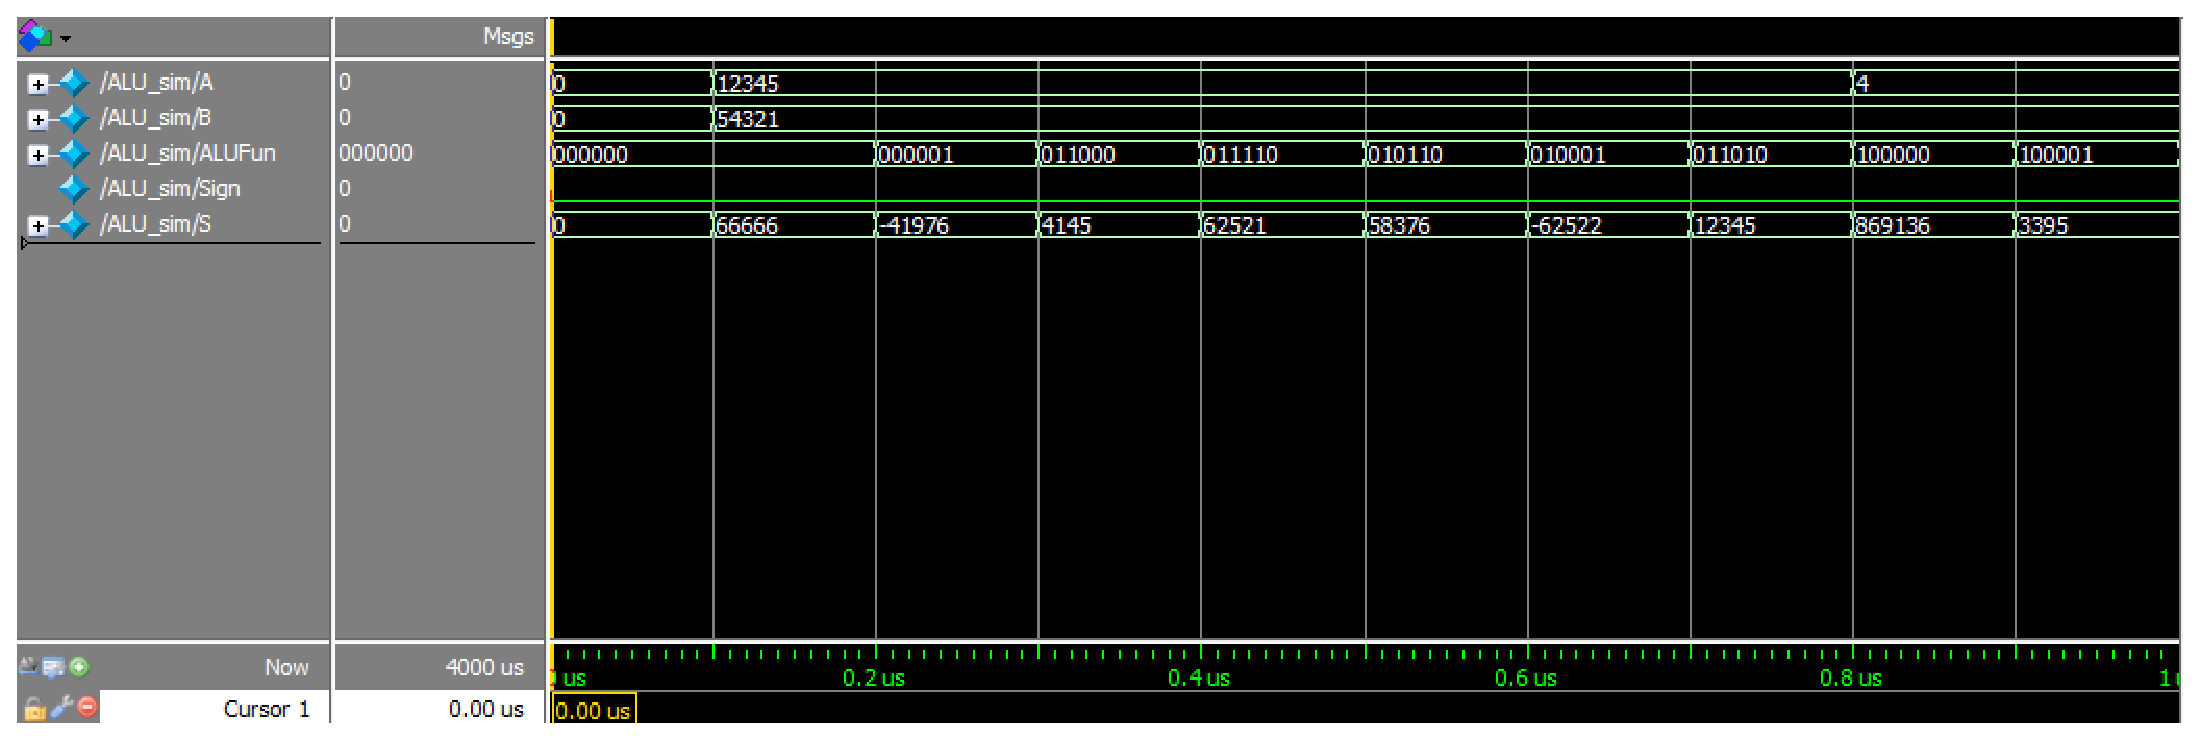
\includegraphics[width = \textwidth]{ALUsim-1.eps}
		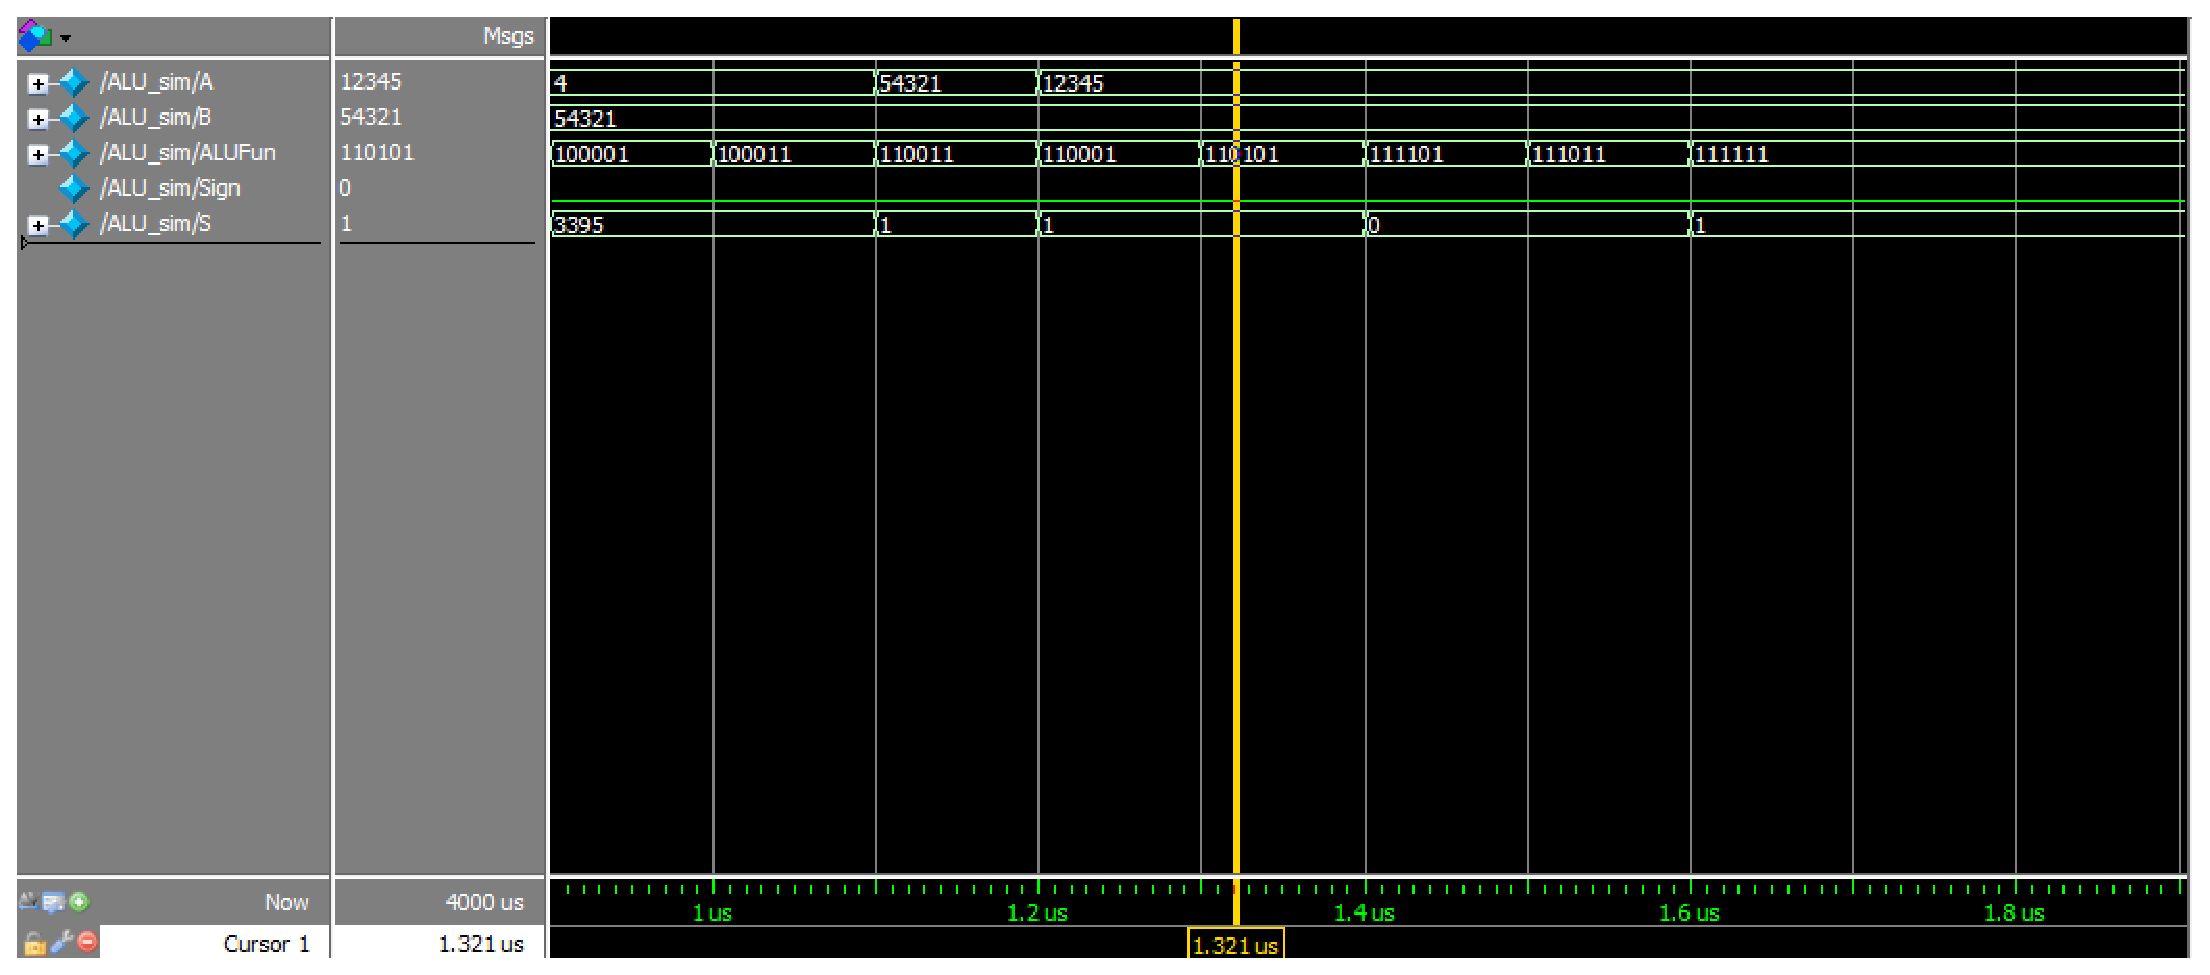
\includegraphics[width = \textwidth]{ALUsim-2.eps}
		\caption{ALU仿真波形}
		\label{simpicture1}
	\end{figure}

	\begin{table}[ht]
		\centering
		\begin{tabular}{c|c}
			\hline
				序号 & 指令 \\
			\hline
				1 & $12345 + 54321 = 66666$ \\
				2 & $12345 - 54321 = -41976$ \\
				3 & $0x3039 \& 0xd431 = 0x1031$ \\
				4 & $0x3039 | 0xd431 = 0xf439$ \\
				5 & $0x3039  \text{ XOR }  0xd431 = 0xe408$ \\
				6 & $\sim(0x3039 | 0xd431) = 0xffff43a$  \\
				7 & $54321 << 4 = 869136$\\
				8 & $54321 >> 4 = 3395$\\
				9 & $54321 >> 4 = 3395$\\
				10 & $54321 == 54321, S = 1$\\
				11 & $54321 != 12345, S = 1$\\
				12 & $12345 < 54321, S = 1$\\
				13 & $12345 > 0, S = 0$ \\
				14 & $12345 > 0, S = 0$ \\
				15 & $12345 > 0, S = 1$ \\
			\hline
		\end{tabular}
		\caption{ALU仿真指令顺序表}
		\label{simtable1}
	\end{table}

	\clearpage

	\subsection{单周期程序仿真}
	\subsubsection{基本四则运算}
	在单周期CPU执行如下程序
	\begin{lstlisting}
addi $t0, $0, 200
addi $t1, $0, -300
add $t2, $t0, $t1
sub $t3, $t0, $t1
	\end{lstlisting}

	得到运行结果如图\ref{simpicture2}。

	\begin{figure}[ht]
		\centering
		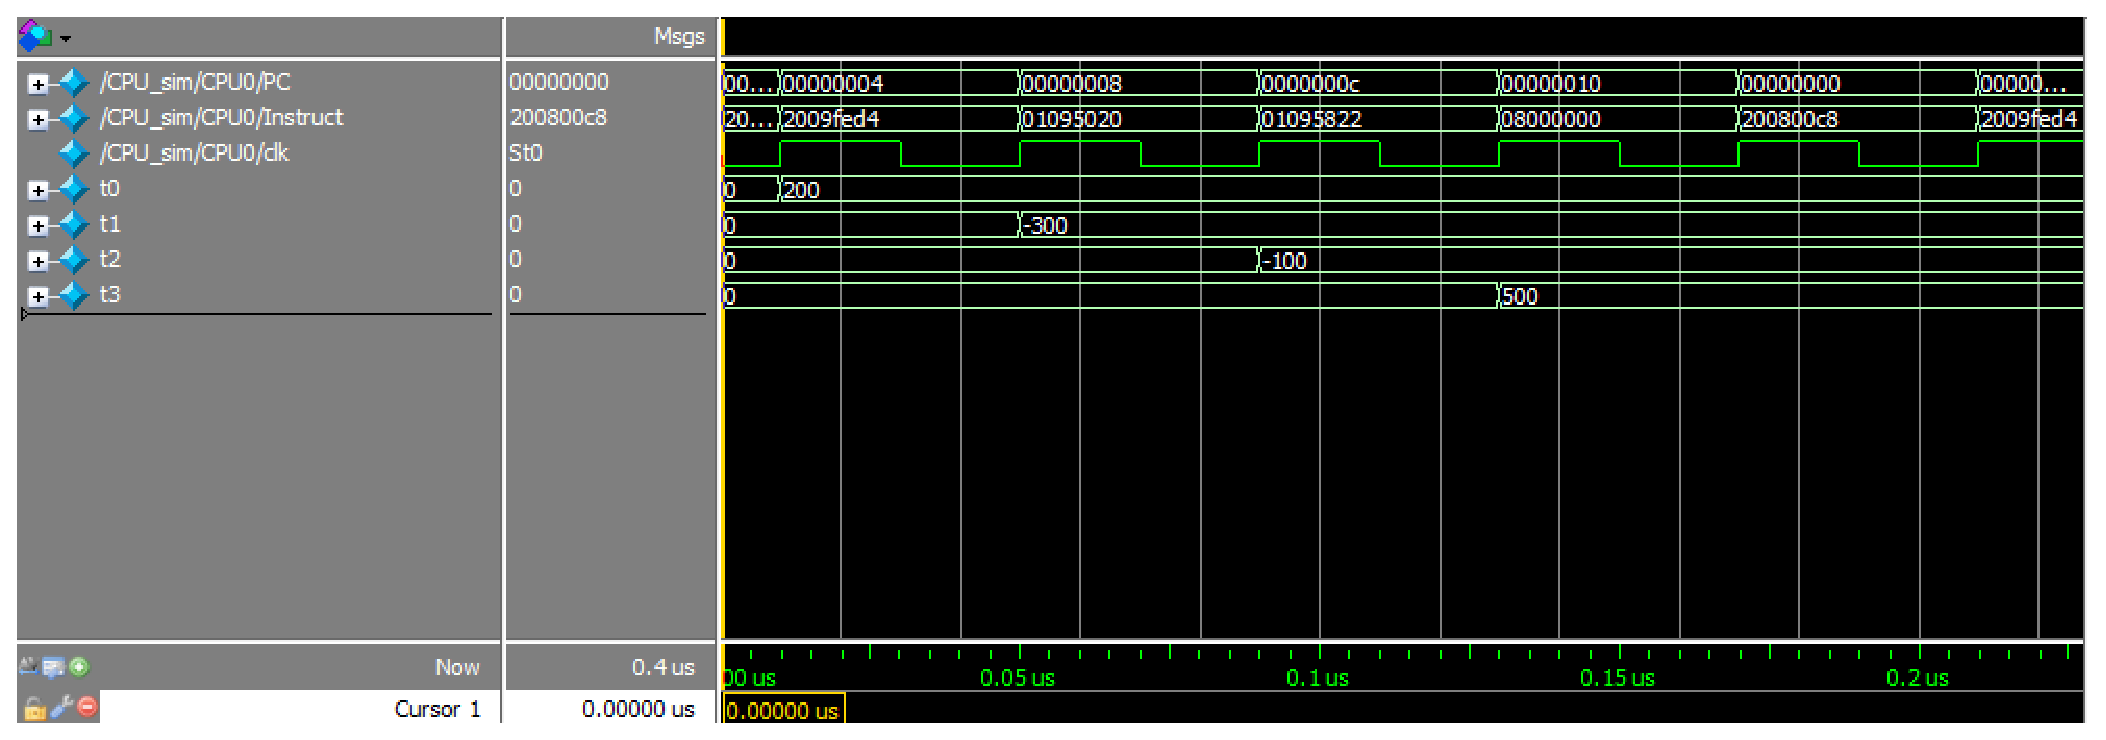
\includegraphics[width = \textwidth]{OneCycleTestWave1.eps}
		\caption{单周期CPU基本运算波形}
		\label{simpicture2}
	\end{figure}

	指令正常完成,对应寄存器正常写入。

	\subsubsection{逻辑运算}
	在单周期CPU中执行如下程序:
\begin{lstlisting}
addi $t0, $0, 0x4321
addi $t1, $0, 0x1234
and $t2, $t0, $t1
or $t3, $t0, $t1
xor $t4, $t0, $t1
addi $t5, $0, 0xffff
andi $t5, $t5, 0x1234	
\end{lstlisting}

得到波形如\ref{simpicture3}。

指令正常完成,对应寄存器正常写入。

	\begin{figure}[ht]
		\centering
		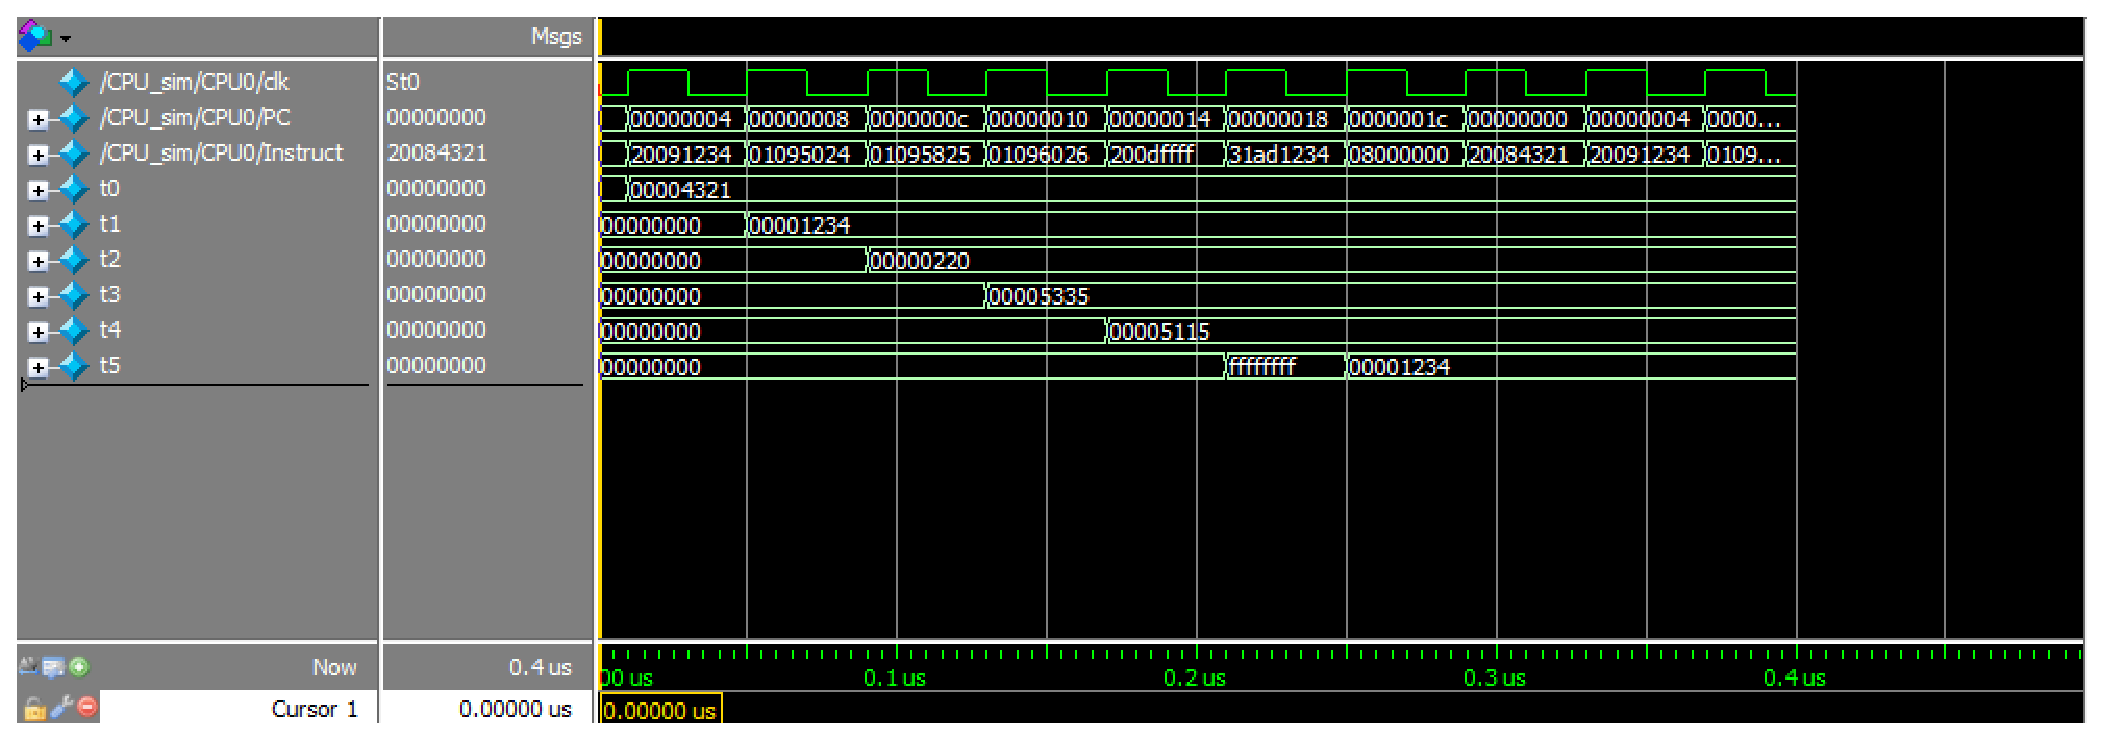
\includegraphics[width = \textwidth]{OneCycleTestWave2.eps}
		\caption{单周期CPU逻辑运算波形}
		\label{simpicture3}
	\end{figure}

	\subsubsection{移位和置位指令}

	在单周期 CPU 中执行如下程序

\begin{lstlisting}
addi $t0, $0, -1234
sll $t1, $t0, 3
srl $t2, $t0, 3
sra $t3, $t0, 3
slt $t4, $t2, $0
slti $t5, $t3, 0
\end{lstlisting}

	得到波形如\ref{simpicture4}。

	\begin{figure}[ht]
		\centering
		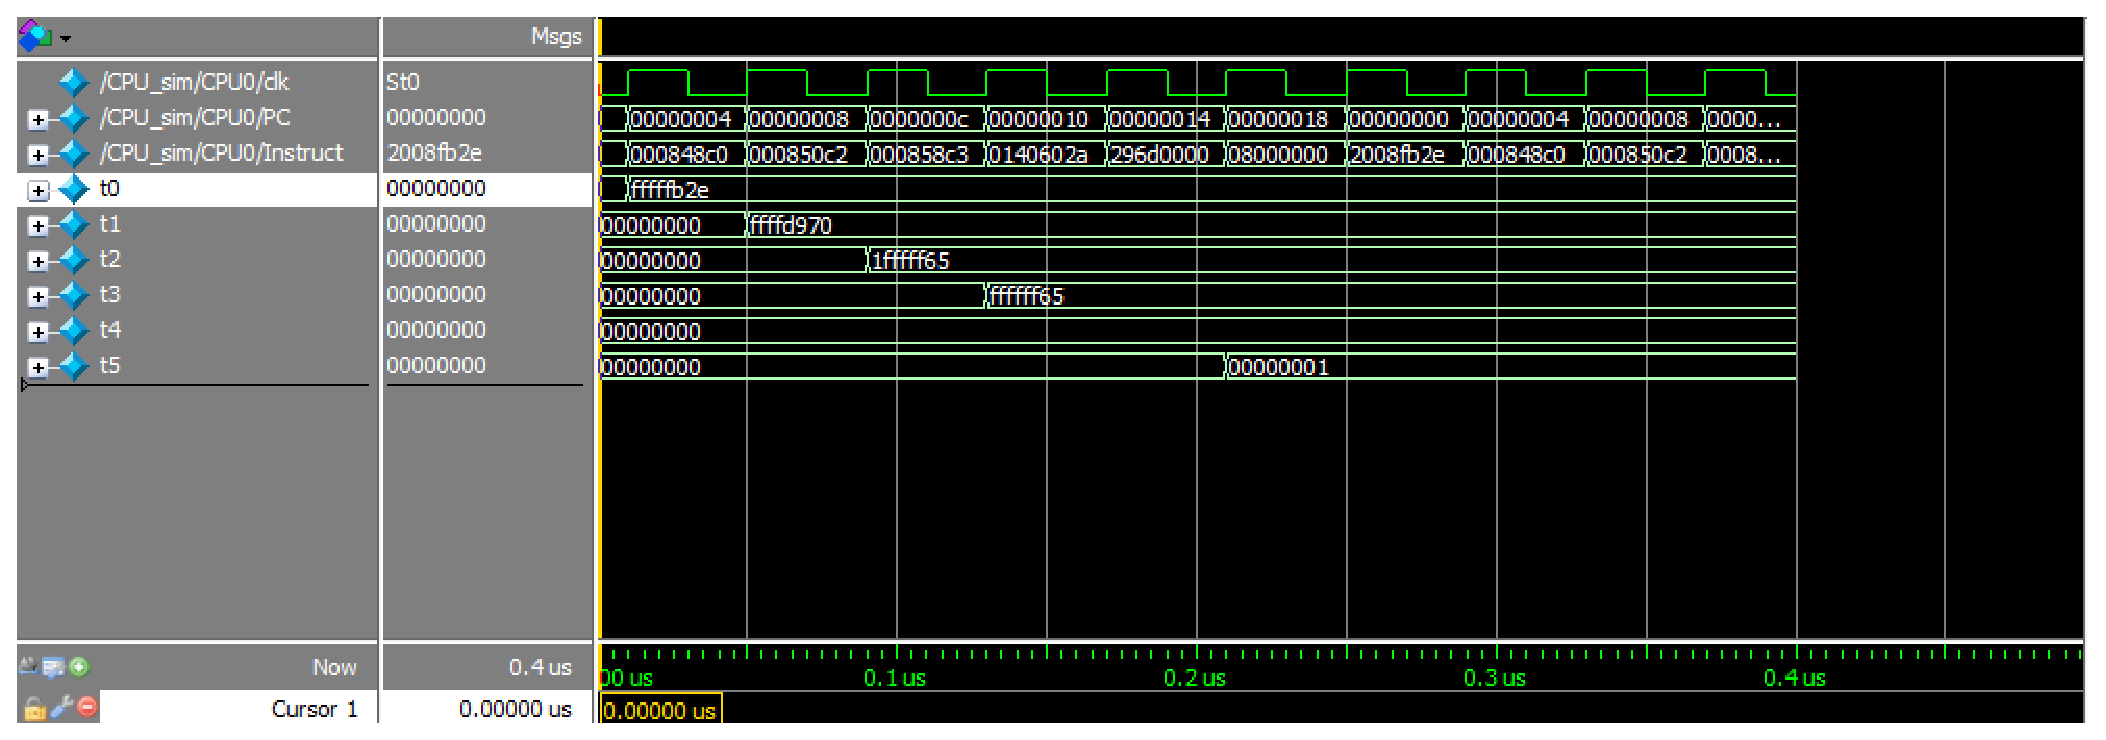
\includegraphics[width = \textwidth]{OneCycleTestWave3.eps}
		\caption{单周期CPU移位与置位运算}
		\label{simpicture4}
	\end{figure}	

	指令正常完成,当使用逻辑右移时,负数将转换为正数,而当使用算数右移时,负数仍然保持符号不变。	

	\subsubsection{跳转指令}

	在单周期 CPU 中执行如下程序

\begin{lstlisting}
A:
beq $0, $0, D
B:
j B
C:
jal E
bne $0, $0, B
j B
D:
j C
E:
jr $ra
\end{lstlisting}	

	得到波形如\ref{simpicture5}。

	\begin{figure}[ht]
		\centering
		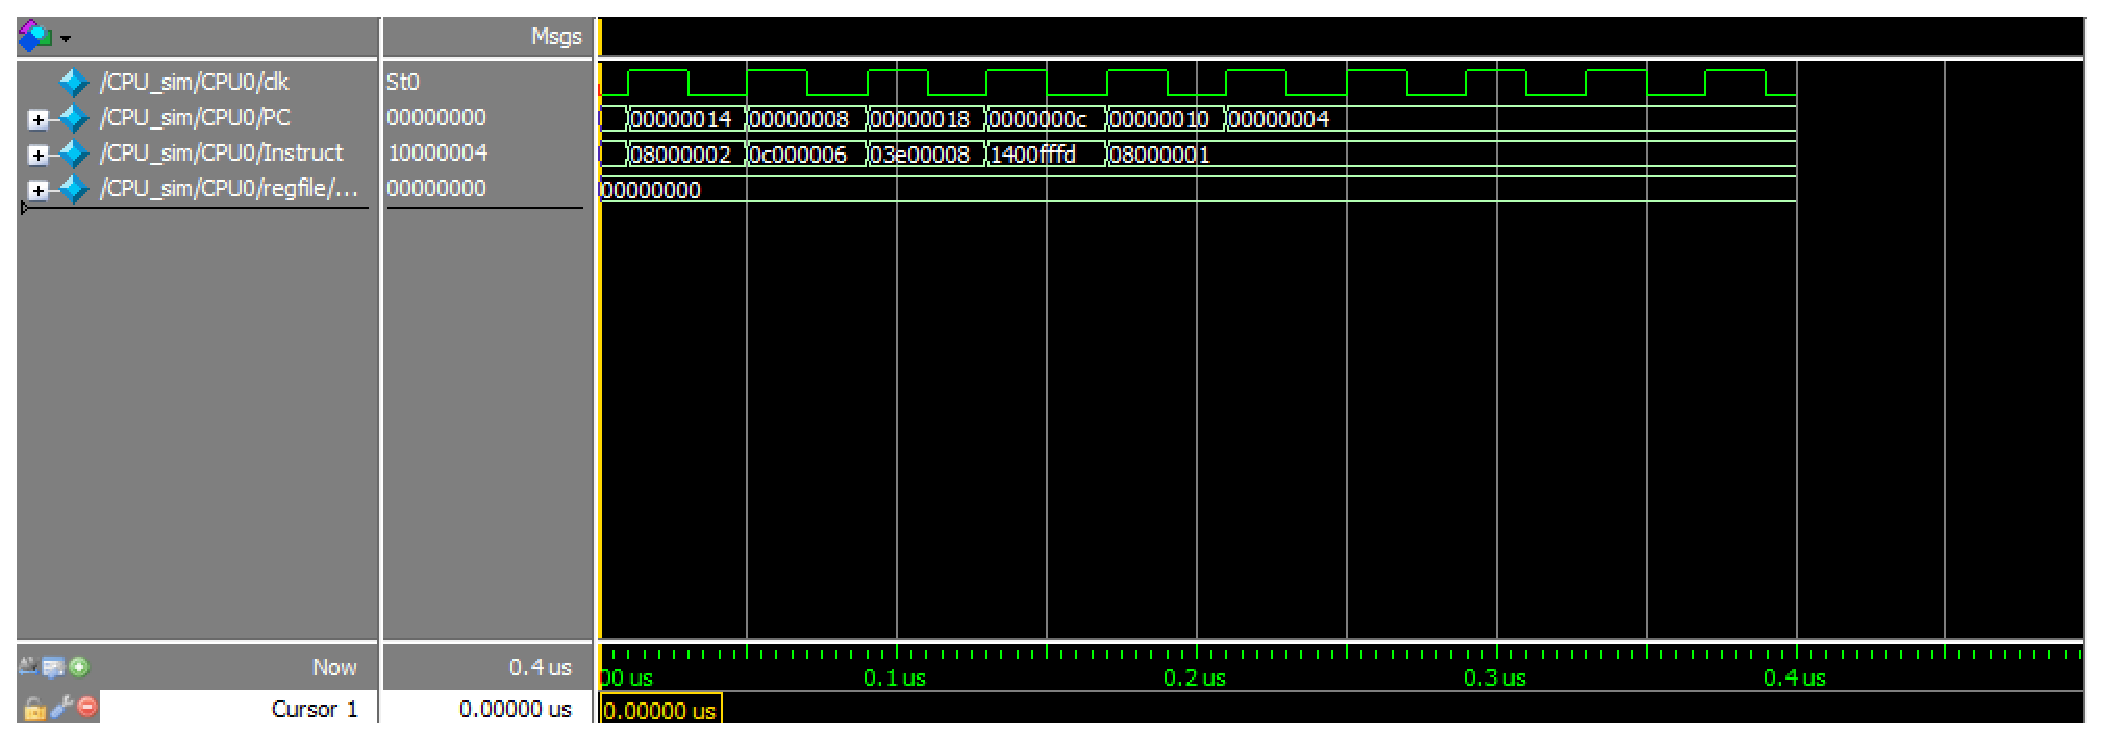
\includegraphics[width = \textwidth]{OneCycleTestWave4.eps}
		\caption{单周期CPU跳转指令}
		\label{simpicture5}
	\end{figure}		
	
	CPU 在多次跳转中正常工作。

	\subsubsection{中断与外设}

	使用实验用最大公约数代码,通过 testbench 模拟串口输入信号,观察中断和串口收发情况。

	当计时器计时完成时,CPU 进入中断处理,最高位置为 1,原程序 PC 被存放在 26 号寄存器中。波形如6。

	\begin{figure}[ht]
		\centering
		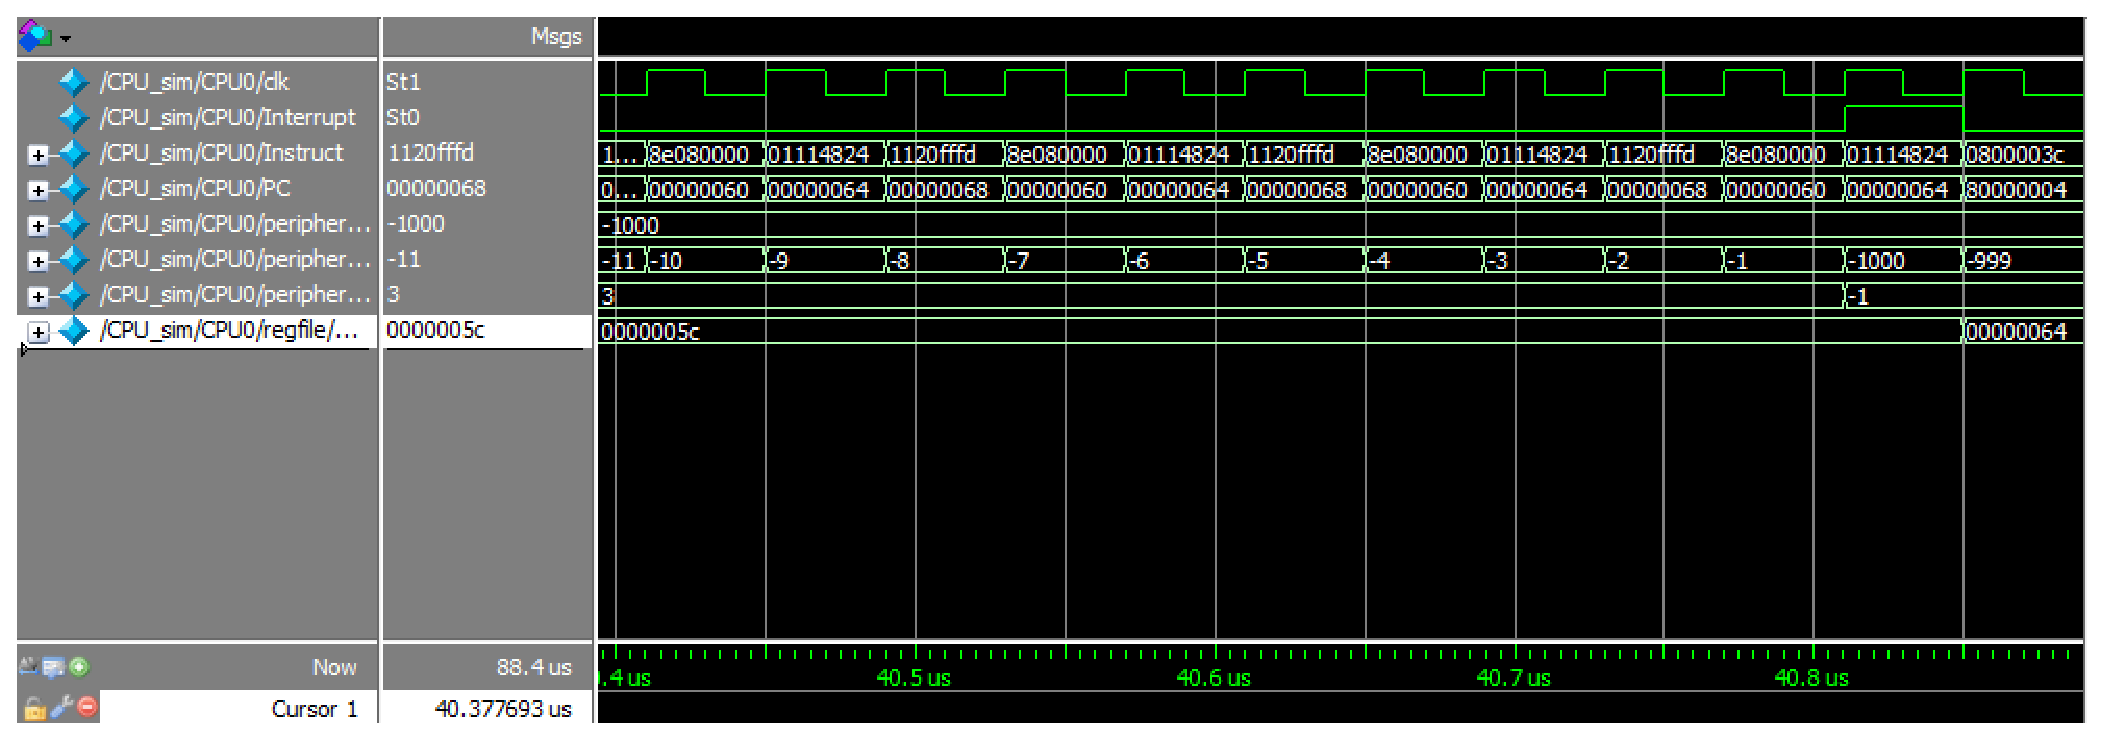
\includegraphics[width = \textwidth]{OneCycleTestWave5.eps}
		\caption{单周期 CPU 中断工作波形}
		\label{simpicture6}
	\end{figure}	

	观察外设整体情况,七段数码管在定时中断中轮流扫描,LED 和串口工作正常,波形如7

	系统正常工作。

	\begin{figure}[ht]
		\centering
		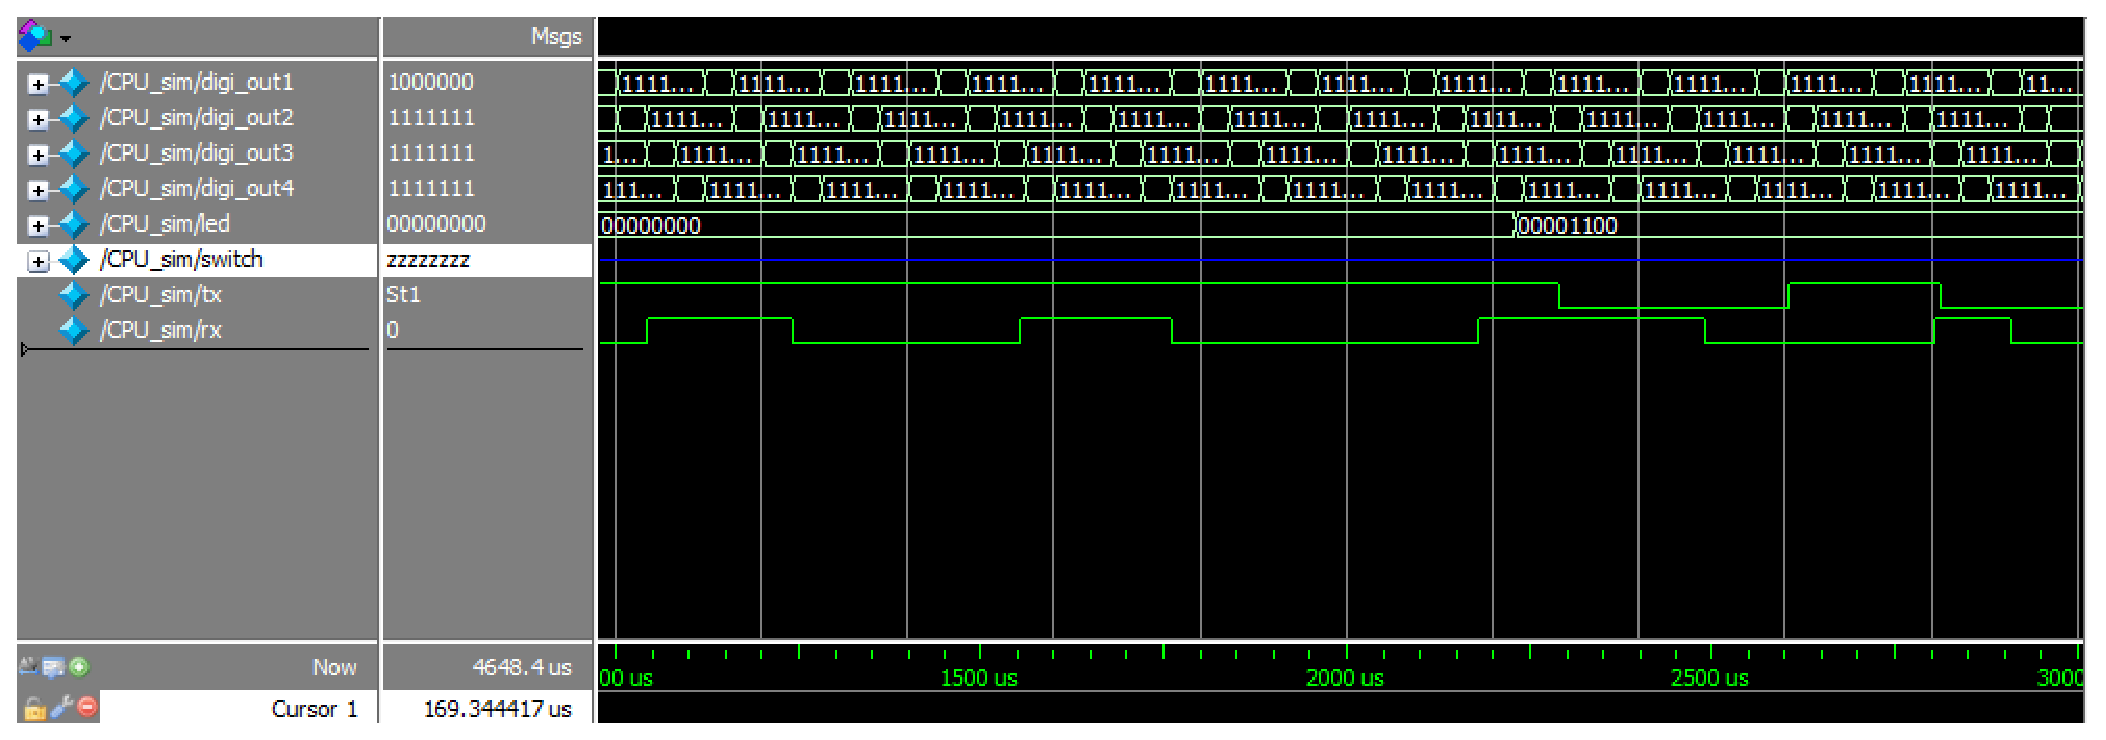
\includegraphics[width = \textwidth]{OneCycleTestWave6.eps}
		\caption{单周期外设与串口工作波形}
		\label{simpicture7}
	\end{figure}	

	\subsection{流水线仿真}
	\subsubsection{冒险与转发}
	在流水线 CPU 中运行如下指令

\begin{lstlisting}
addi $t0, $0, 1234
add $t1, $t0, $0
sub $t2, $0, $t0
\end{lstlisting}

	仿真波形如\ref{simpicture8}。

	\begin{figure}[ht]
		\centering
		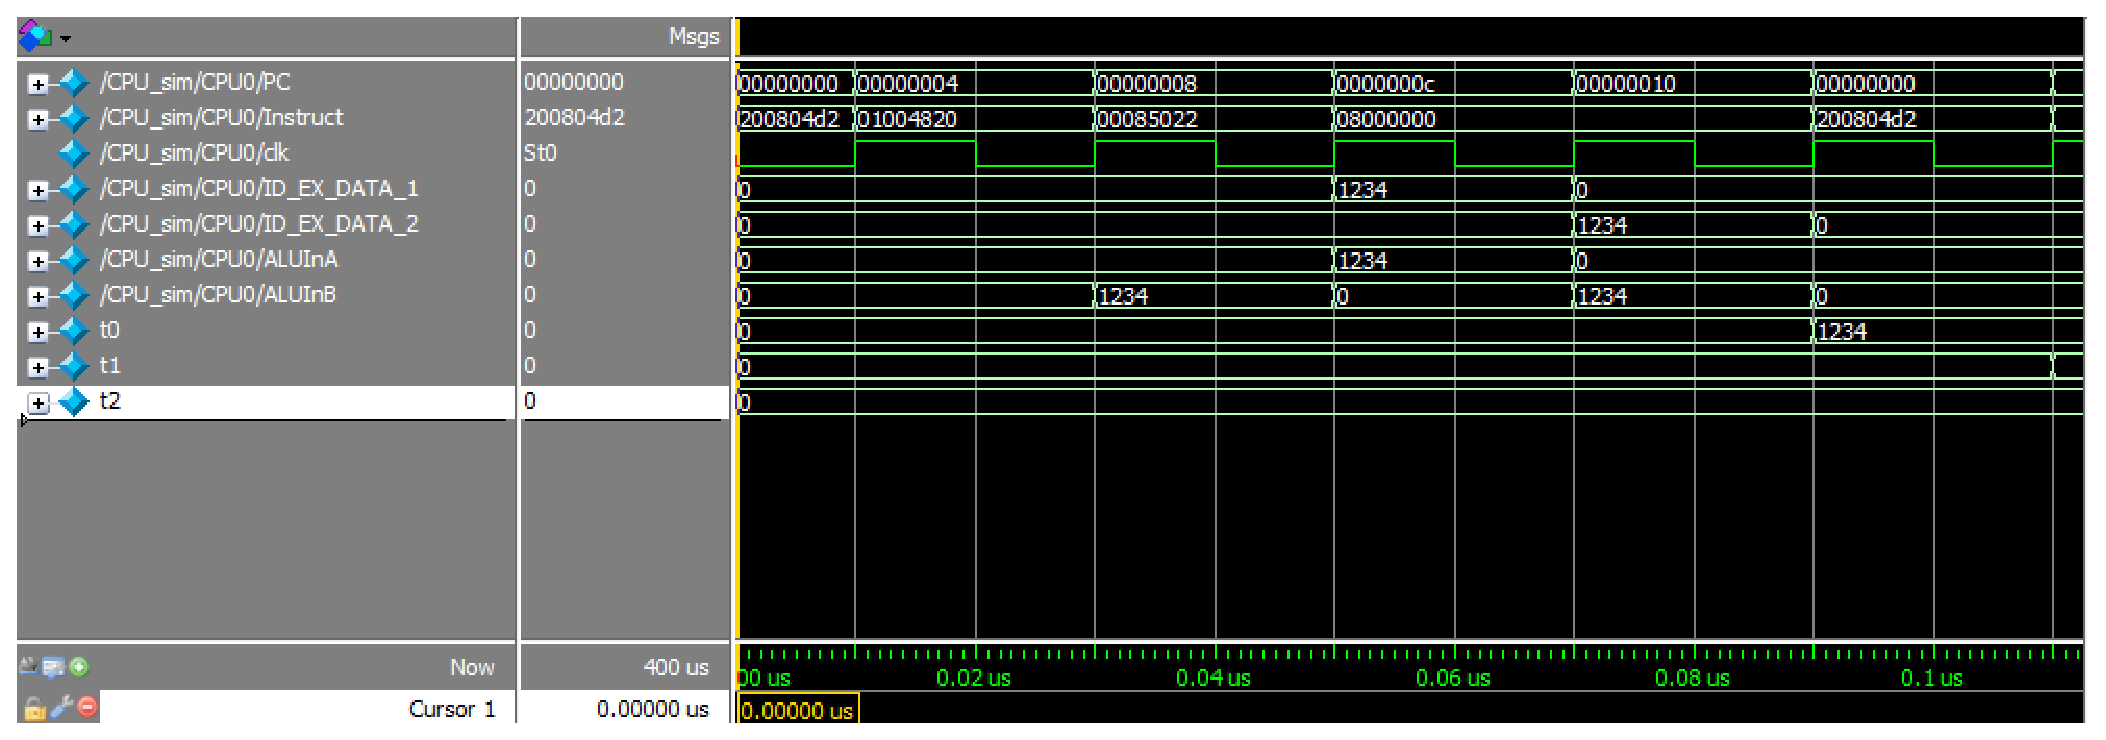
\includegraphics[width = \textwidth]{PipelineTestWave1.eps}
		\caption{流水线冒险与转发}
		\label{simpicture8}
	\end{figure}		

	可以看到虽然上一条指令的结果还未写入寄存器,但是通过 EX/MEM 和 MEM/WB 两层寄存器的转发,仍然可以获得正确的结果。

	\subsubsection{load-use处理}
	
	在流水线 CPU 中运行如下指令

	\begin{lstlisting}
addi $s0, $0, 0x4000
sll $s0, $s0, 16
lw $t0, 0($s0)
add $t1, $t0, $t0
add $t2, $t0, $t0	
	\end{lstlisting}
	
运行时波形如\ref{simpicture9}。

	\begin{figure}[ht]
		\centering
		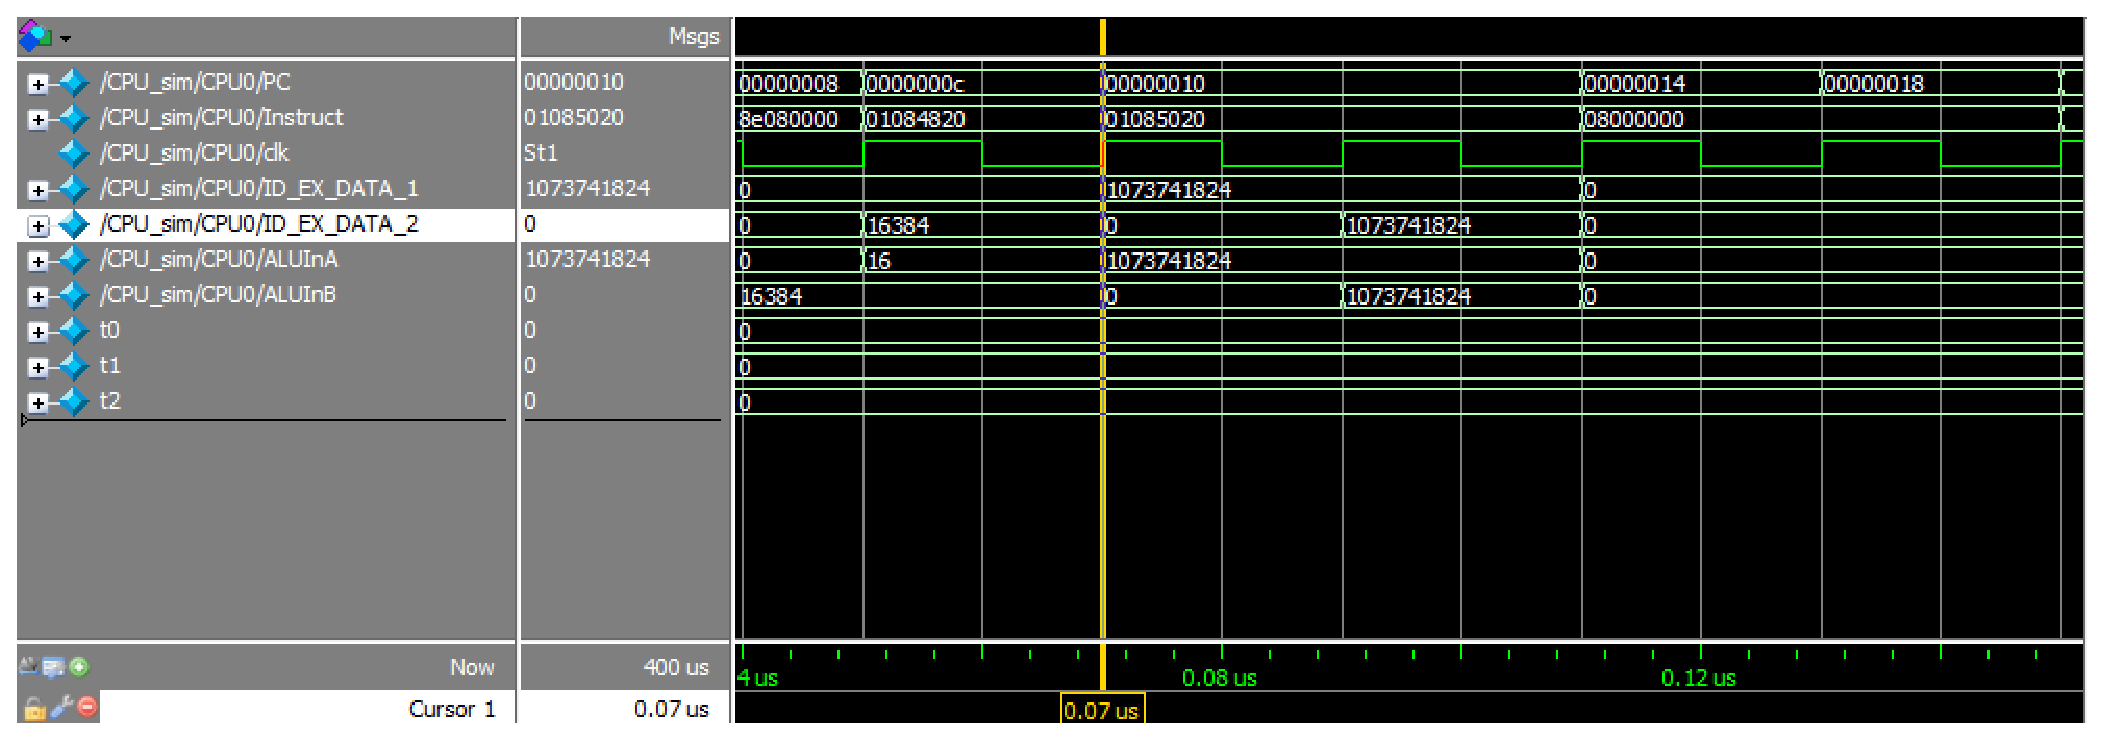
\includegraphics[width = \textwidth]{PipelineTestWave2.eps}
		\caption{ load-use 处理}
		\label{simpicture9}
	\end{figure}

当地址为 0x0000000C 的指令,发现其出现 load-use 类竞争时,会阻塞一个周期等待 lw 指令执行完成。通过这一处理,该指令可以获得正确的数据。

	\subsubsection{branch 指令}

	在流水线CPU中运行如下指令
	\begin{lstlisting}
beq $0, $0, A
addi $t0, $0, 1
A:
addi $t0, $0, 2
	\end{lstlisting}

	运行时波形如\ref{simpicture10}。

	\begin{figure}[ht]
		\centering
		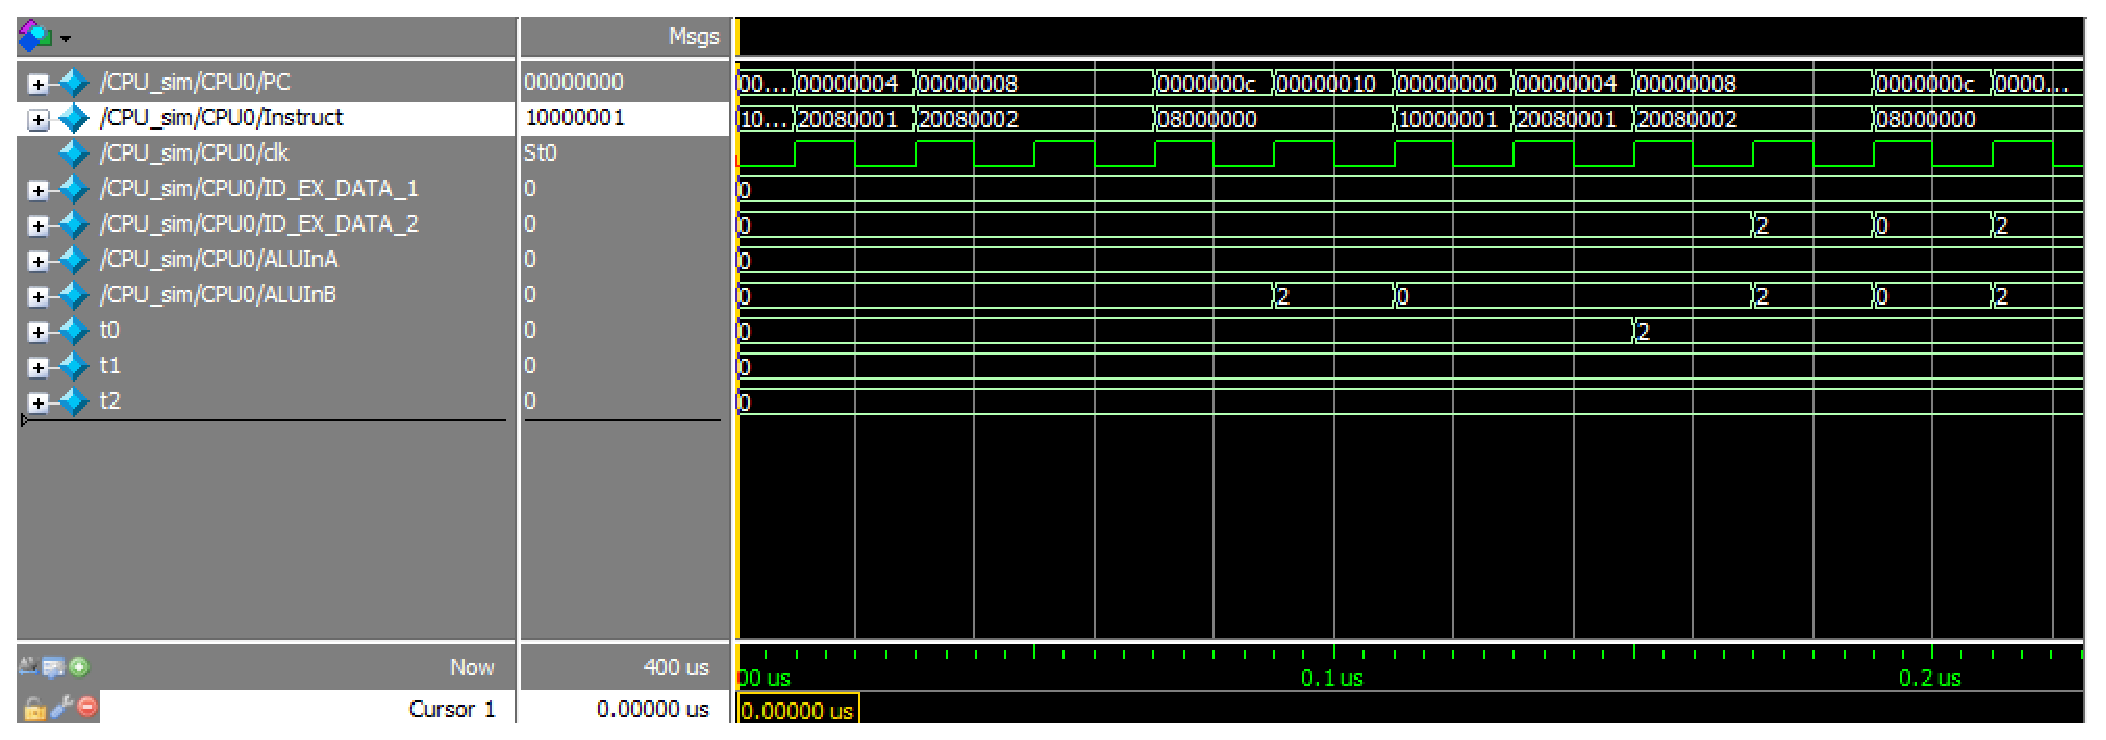
\includegraphics[width = \textwidth]{PipelineTestWave3.eps}
		\caption{branch 处理}
		\label{simpicture10}
	\end{figure}
	当 beq 语句执行到 ex 阶段时,判断跳转为真并将当前 IF 和 ID 阶段的两条指令清除,将跳转
目标,此处为 0x00000008 放入 PC 中。执行跳转后的目标指令。

	\subsubsection{j指令}
	
	在流水线中运行如下指令

\begin{lstlisting}
j A
addi $t0, $0, 1
addi $t0, $0, 2
addi $t0, $0, 3
A:
addi $t0, $0, 10
j B
B:
j B
\end{lstlisting}

	得到波形如\ref{simpicture11}。

	\begin{figure}[ht]
		\centering
		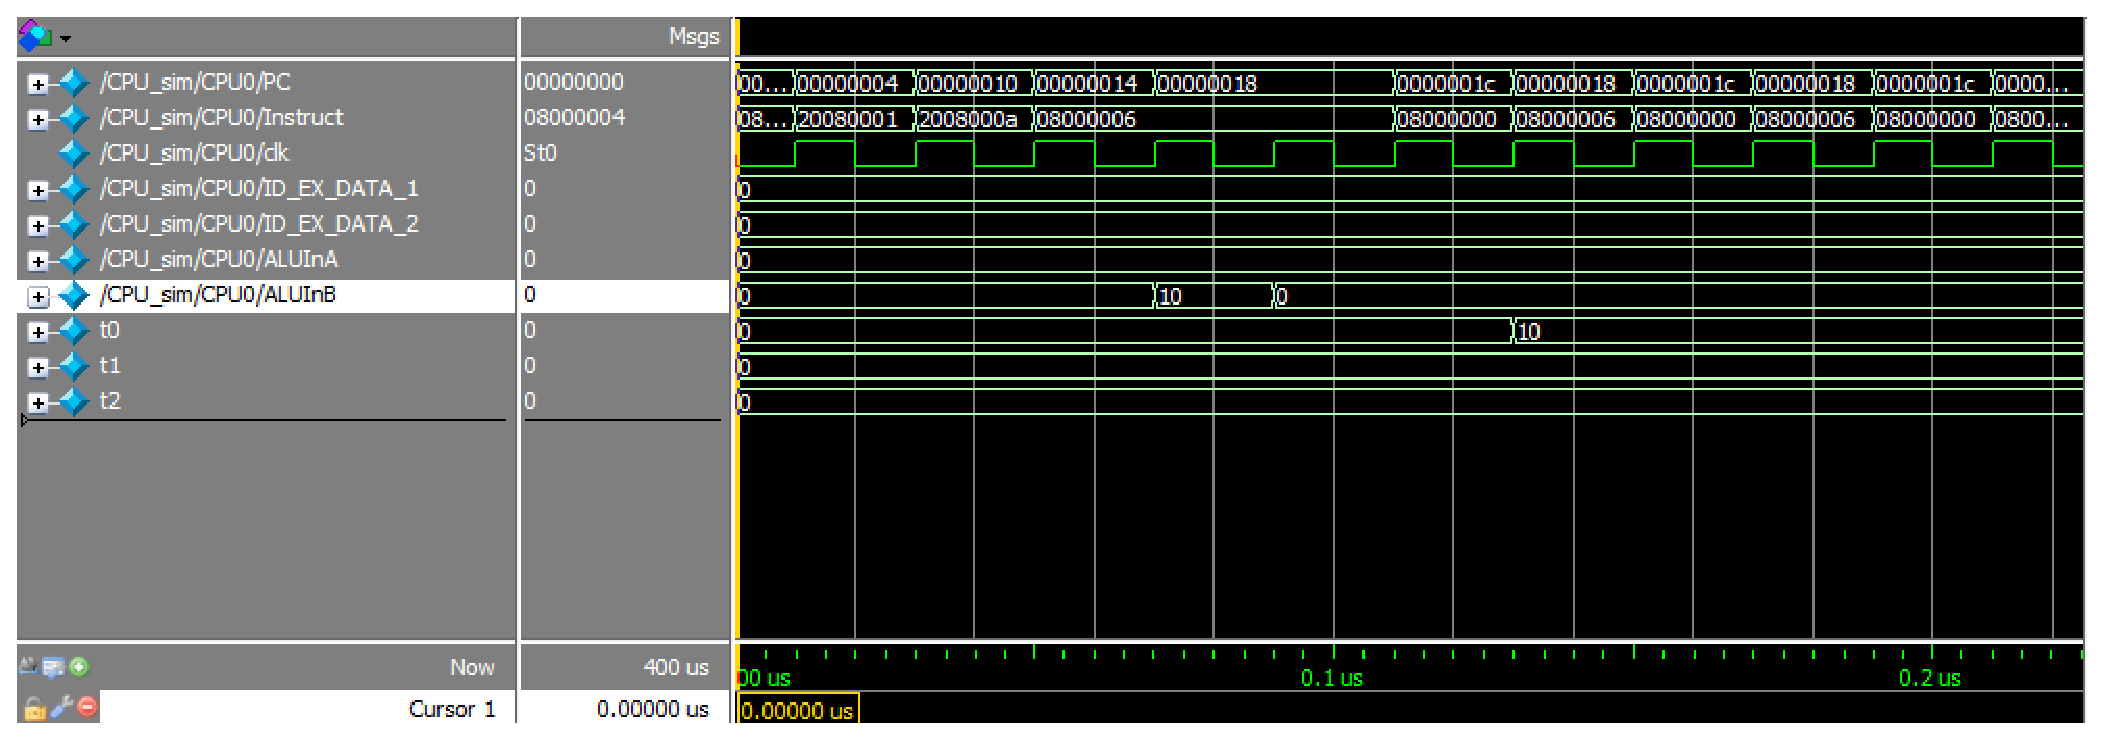
\includegraphics[width = \textwidth]{PipelineTestWave4.eps}
		\caption{j 处理}
		\label{simpicture11}
	\end{figure}

	虽然 j 指令之后的一条指令进入了 IF 阶段,但其从未被执行,j 指令会将其控制信号全部清零后跳转到目标地址。

	\subsubsection{中断和外设}

	使用实验用最大公约数代码,通过 testbench 模拟串口输入信号,观察中断和串口收发情况。

	中断波形如\ref{simpicture12}。在 0x00000068 指令触发中断后,0x00000068 指令并未被实际执行,系统进入中断处理程序,中断处理程序结束后的返回地址将在完成五级流水后存入寄存器中。返回地址与触发中断时执行的指令直接相关。

	\begin{figure}[ht]
		\centering
		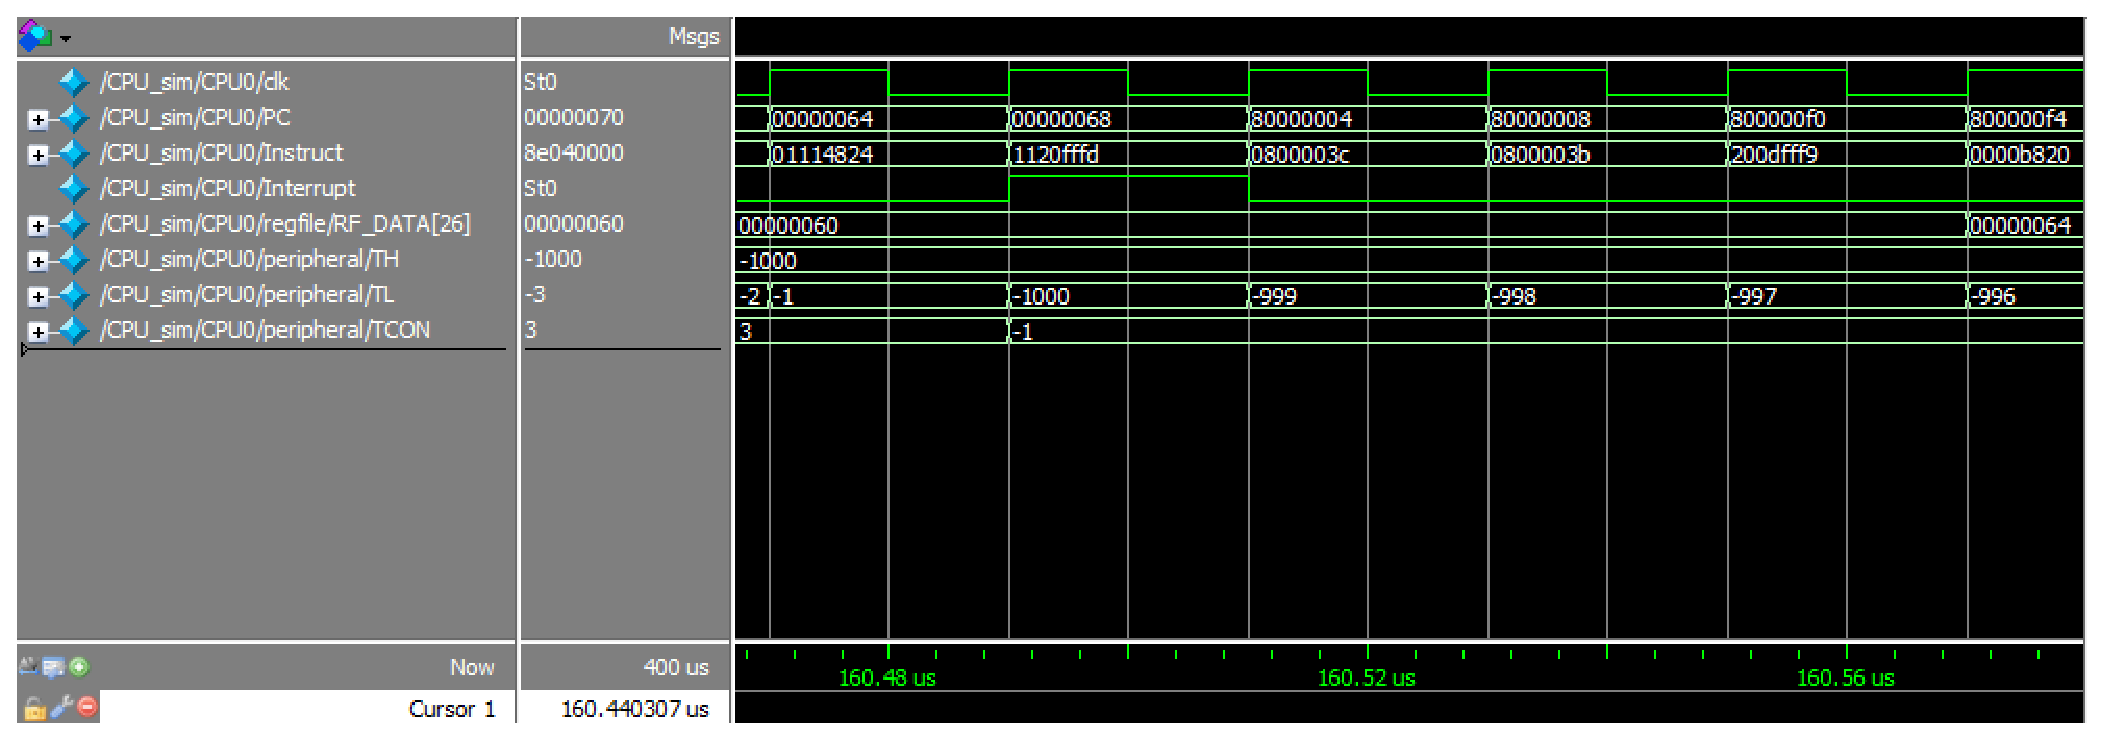
\includegraphics[width = \textwidth]{PipelineTestWave5.eps}
		\caption{中断处理}
		\label{simpicture12}
	\end{figure}

	外设工作情况如图\ref{simpicture13}。

	\begin{figure}[ht]
		\centering
		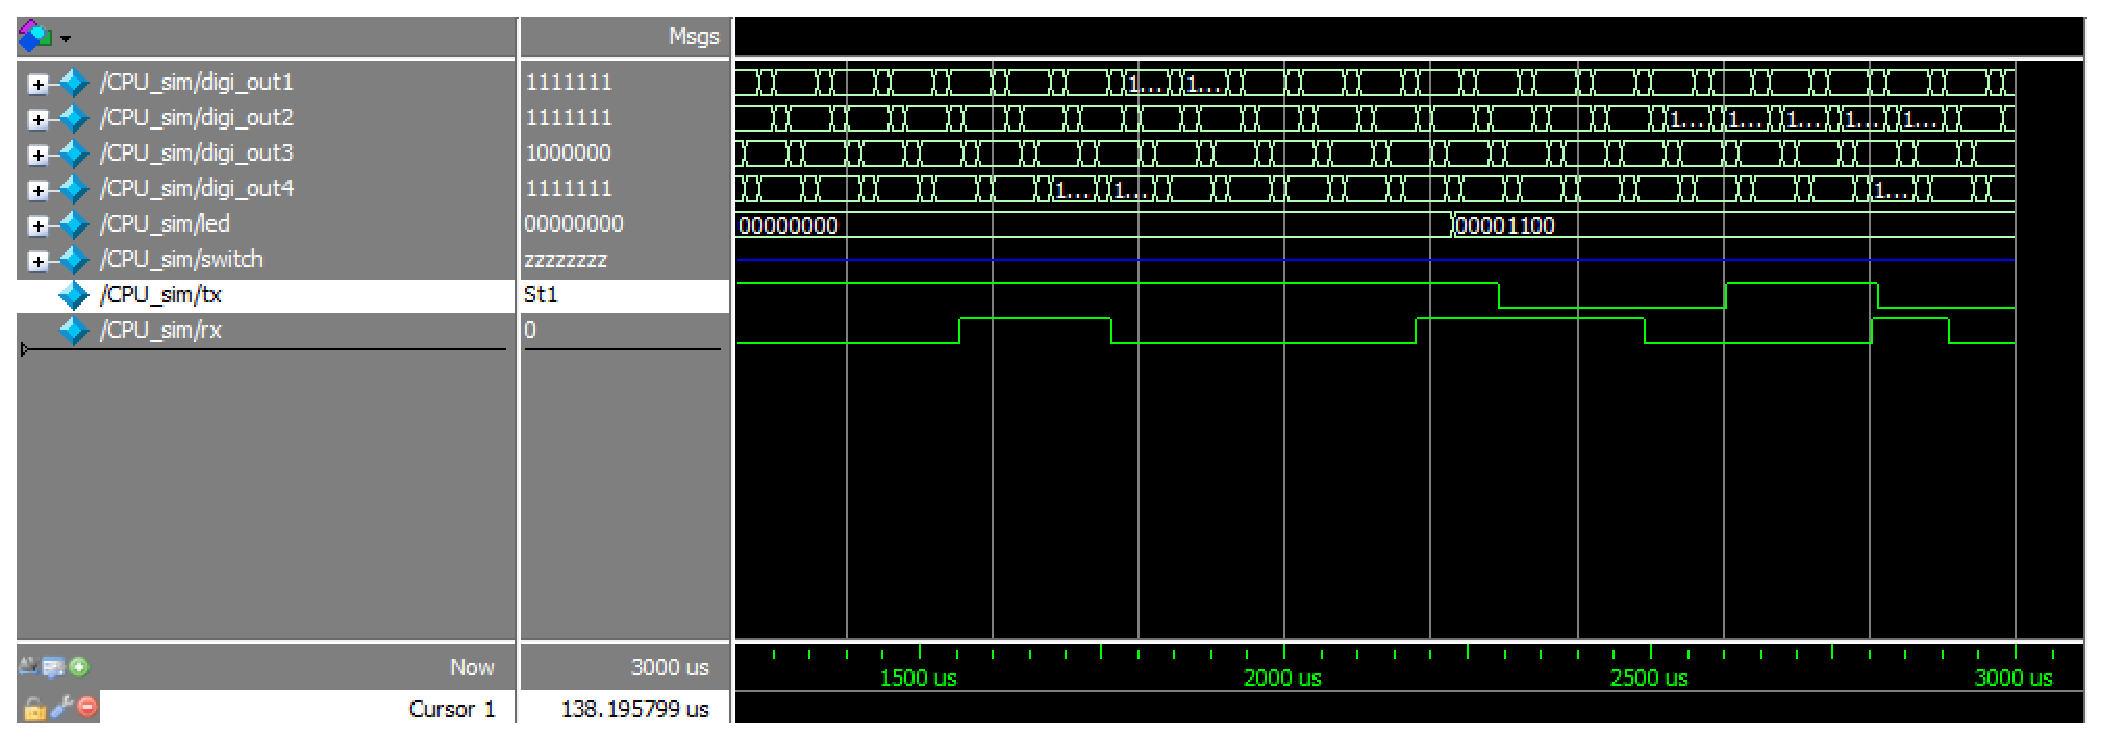
\includegraphics[width = \textwidth]{PipelineTestWave6.eps}
		\caption{流水线 CPU 外设工作情况}
		\label{simpicture13}
	\end{figure}	

	\section{综合情况}
	单周期各项性能指标如下:
	\begin{center}
		\begin{tabular}{|c|c|}
		\hline
		性能指标 & \\
		\hline
		Total Logic Elements & 4498(14\%) \\
		Total Registers & 3772(11\%) \\
		Total Pins & 48(10\%) \\
		Restricted Fmax & $41.55 MHz$ \\  
		\hline
		\end{tabular}
	\end{center}
	
	流水线各项性能指标如下:
	\begin{center}
		\begin{tabular}{|c|c|}
		\hline
		性能指标 & \\
		\hline
		Total Logic Elements & 3803(11\%) \\
		Total Registers & 3695(11\%) \\
		Total Pins & 48(10\%) \\
		Restricted Fmax & $88.0 MHz$ \\  
		\hline
		\end{tabular}
	\end{center}
	\section{硬件调试情况}
\begin{itemize}
	\item  七段数码管正确扫描显示待计算数据,LED 灯正确显示结果
	\item  串口收发正确进行
	\item  运算任务正确完成 
\end{itemize}
	\section{思想体会}

	\subsection{王敏虎}

	在团队中,我主要负责汇编器、汇编代码、外设相关代码和testbench的编写。

	在实验中,最大的收获是理解了中断对于CPU的意义,以及CPU如何通过中断完成I/O操作。对于CPU将外设抽象为存储地址这一工程实践有了初步的认识。同时,通过测试CPU代码,了解了CPU开发中比较容易出错的地方。例如在流水线CPU中断设计中,最初中断始终不成功,在反复比对波形后,最终发现是存入寄存器的地址不对,进而发现此处应当根据执行的指令对存储地址进行判断。
\end{document}